In this thesis we will study linear temporal logic and its connection to automata theory. Linear temporal logic (LTL) was, among other people, introduced by Pnueli in 1977. Pnueli introduced LTL in order to specify and verify \textit{reactive and concurrent systems}. Temporal logic formulas can describe a property of these systems but it is also important to decide if this property holds in a certain model. That is where automata theory is helpful. In order to solve the decision problem for temporal logics, a formula is translated into an automata on infinite words. Then satisfiability of a formula is equivalent to non-emptiness of the language of the automaton \cite{sep-logic-temporal}. Next to the general linear temporal logic there are also numerous extensions and varieties such as branching time temporal logic and the linear time $\mu$-calculus which we will study in this thesis.

Linear temporal logic uses infinite models on the natural numbers. Such model can be viewed as describing the subset of propositional letters that are true at the time step given by a natural number. Visually this can be represented in figure \ref{fig:modelexample}.
\begin{figure}[h!]
 \centering
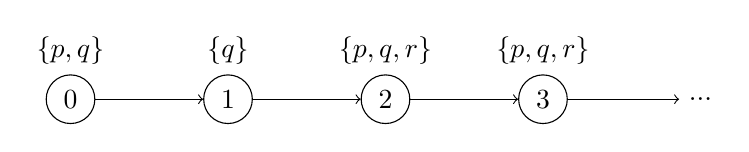
\begin{tikzpicture}
  % Define the nodes
  \node[circle, draw] (0) at (6,0) {$0$};
  \node[circle, draw] (1) at (8,0) {$1$};
  \node[circle, draw] (2) at (10,0) {$2$};
  \node[circle, draw] (3) at (12,0) {$3$};
  \node (4) at (14,0) {$...$};

  % Draw arrows between nodes to represent the accessibility relation
  \draw[->] (0) -- (1);
  \draw[->] (1) -- (2);
  \draw[->] (2) -- (3);
  \draw[->] (3) -- (4);

  % Optional: Add labels or other decorations
  \node[above] at (0.north) {$\{p, q\}$};
  \node[above] at (1.north) {$\{q\}$};
  \node[above] at (2.north) {$\{p, q, r\}$};
  \node[above] at (3.north) {$\{p, q,r\}$};
\end{tikzpicture}
\caption{Example of a linear model, where we for example say that $p$ and $q$ hold at time step $0$.}
\label{fig:modelexample}
\end{figure}
% \vspace{-3mm}

\noindent In the context of automata these models are usually viewed as infinite $\omega$-words over the alphabet $\PP(\Psf)$ where $\Psf$ is the set of propositional letters. When using Linear Temporal Logic to describe the behaviour of concurrent programs Lamport \cite{lamport1983whatgood} introduced the concept of stuttering in 1983. He argues that a formula should not describe the number of steps needed to reach the next state. He argues that this is a desired and natural property for a temporal logic to have. We can more formally define this notion of \emph{stuttering} as follows. Informally stuttering means repeating letters and removing consecutive occurences from the word. We say that two words are stutter-equivalent if they can be transformed into each other by stuttering.
For example the words $w=aabbcc$ and $w'=abbbccc$ are stutter-equivalent (notation $w\sim_s w'$) since we can remove one $a$ from $w$ add a $b$ and add a $c$ to $w$ to get $w'$. But $w=aabbcc$ and $w=aadcc$ are not stutter-equivalent since you cannot add new letters or remove all consecutive occurrences of a letter.
A language is \emph{stutter-invariant} if for every $w, w'\in \Sigma^\omega$ (where $\Sigma^\omega$ is the set of infinite words over alphabet $\Sigma$) with $w\sim_s w'$ stutter equivalent we have

\[
 w\in\LL \text{ if and only if } w'\in\LL.
\]

Lamport argues that any temporal logic should only have stutter-invariant languages. In this thesis we will study the Linear Time $\mu$-calculus ($\mutl$), an extension of LTL where the fixpoint operators $\mu$ and $\nu$ are added. It is shown by  Amélie Gheerbrandt and Balder ten Cate \cite{gheerbrandt2009craiginterpolation} that $\mutl(U,R)$ is the stutter-invariant fragment of the Linear Time $\mu$-calculus. We also know that $\mutl$ is $\omega$-regular which means that for every $\phi\in\mutl$ there exists an $\omega$-automaton that defines exactly the language of $\phi$ \cite{demri2016temporal}. In this thesis we will work with Non-Deterministic Parity Automaton (\npa) which are a specific type of $\omega$-automata. We specifically choose the parity condition since this allows for a natural translation of the fixpoint formulas. We also know that there exists a procedure to check if a $\omega$-regular language is stutter-invariant. For example Thibaud Michaud and Alexandre Duret-Lutz \cite{michaud2015practical} give a procedure to determine if a Nondeterministic Transition Büchi automaton has a stutter-invariant language.

In this thesis we will alter the construction of \cite{michaud2015practical} to work with \npa s and use this to prove, just like Gheerbrandt and Ten Cate, that $\mutl(U,R)$ is the stutter-invariant fragment of $\mutl$. The original plan of this project was to provide a proof that for every $\mutl$ formula $\phi$ there exists an equivalent \npa\, and vice versa. Then to provide a construction to determine the stutter-closure of an \npa\, and use this construction to prove that $\mutl(U,R)$ is the stutter-invariant fragment of $\mutl$. This plan was too ambitious for a Bachelor project so the scope of this thesis is smaller. We will first provide a translation for a $\mutl$ formula a a \npa. For a \npa\, $\A$ we will provide a construction to obtain an \npa\, $\A^s$ that recognizes the stutter-closure of the language of $\A$. With this construction we will give the sketch of the proof that $\mutl(U,R)$ is the stutter-invariant fragment of $\mutl$. We will also explain the difficulties why we did not find a full proof in Section \ref{section:mutlstutinvariant}.

In addition we will define parity automata and prove the stutter-closure construction on these automata in the formal proof assistant $\lean$. Due to time-issues we will only formalize part of the proof of Theorem \ref{thm:stutterclosednpa} in $\lean$. Obviously this computer verified proof of our proof will help our belief of the correctness of this proof. But formalization in $\lean$ is also a useful skill to have in the current-day mathematics world. More motivation about formalizing in general and in $\lean$ specifically will be given in Chapter 5.

For this thesis we used the lecture notes \textit{Lectures on the Modal $mu$-calculus} of Yde Venema \cite{venema2024modalmucalculus} as the basis for our definition of the linear time $\mu$-calculus. We will refer to these in the specific sections. For the definition of parity and alternating parity automaton we used the textbook \textit{Temporal Logics in Computer Science} of Demri, Goranko and Lange \cite{demri2016temporal} and will also refer to these in the specific sections. We also used the textbook \textit{Automata, Logics, and Infinite Games} \cite{gradel2003automata} as background material. In addition to the textbooks as sources for our definitions we explored the existing literature on this topic. We directly used theorems from the literature but also used ideas from existing articles for the theorems in this thesis.

The thesis is structured as follows. Chapter 2 provides the necessary background about $\mutl$, parity-automata and stuttering. In Chapter 3 we provide a translation of $\mutl$ to parity automata and prove that this translation is correct. In Chapter 4 we develop a construction to determine whether a $\omega$-automaton is stutter-invariant and give an overview of the way to prove that every formula in $\mutl(U,R)$ is stutter-invariant. Lastly in Chapter 5 we will describe the formalization process in $\lean$. As the subjects of this thesis: logic, automata and formalization in $\lean$ not only lie on the boundary of Mathematics and Computer science but actually in the intersection of both fields it is less meaningful to define a Mathematical and a Computer Science part of this thesis. Formally the supervision of the Mathematics part of this thesis was done by Yde Venema. He supervised the theory and proofs of logic and automata. Malvin Gattinger, as Computer Science supervisor, supervised the formalization in $\lean$.


% Oude versie:::
% In this thesis we will study Linear time temporal fixpoint logic or Linear Time $\mu$-calculus ($\mutl$) and it's stutter-invariant fragment. Linear Time $\mu$-calculus is a logic that describes properties on a linear model with both temporal and fixpoint logic. \textcolor{red}{Wil ik hier meer uitleggen over mutl, of is dit goed?} It is an extension of the normal linear time logic with added fixpoint operators. Such a logic describes languages of infinite $\omega$-words, such that these words satisfy a formula. \textcolor{red}{Dit is vaag, moet iets duidelijker}.
%
% On these $\omega$-words we can define the notion of stuttering.Intuitively stuttering means repeating letters and removing consecutive occurences from the word. We say that two words are stutter-equivalent if they can be transformed into each other by stuttering.
% For example the words $w=aabbcc$ and $w'=abbbccc$ are stutter-equivalent (notation $w\sim_s w'$) since we can remove one $a$ from $w$ add a $b$ and add a $c$ to $w$ to get $w'$. But $w=aabbcc$ and $w=aadcc$ are not stutter-equivalent since you cannot add new letters or remove all consecutive occurences of a letter.
% A language is \emph{stutter-invariant} if for every $w, w'\in \Sigma^\omega$ (where $\Sigma^\omega$ is the set of infinite words over alphabet $\Sigma$) with $w\sim_s w'$ stutter equivalent we have
%
% \[
%  w\in\LL \text{ if and only if } w'\in\LL.
% \]
% According to Lamport \cite{lamport1983whatgood} stutter-invariancy is a desired and natural property of a temporal logic. He introduced temporal logic to study concurrent programs and he argues that when one wants to talk about the next state of the program you actually mean the next state where a significant change occurs. Therefore there should be no difference between $aaac$ and $aac$ since in both cases the next significant change after $a$ is $c$. That means we have to use a logic that is stutter-invariant, and for this we want to check if a specific logic is stutter-invariant.
%
% It is shown by  Amelie Gheerbrandt and Balder ten Cate \cite{gheerbrandt2009craiginterpolation} that $\mutl(U,R)$ is the stutter-invariant fragment of the Linear Time $\mu$-calculus. We also know that  $\mutl$ is $\omega$-regular which means that for every $\phi\in\mutl$ there exists an $\omega$-automaton that defines exactly the language of $\phi$, [Bron]. In this thesis we will work with Non-Deterministic Parity Automaton (NPA) which are a specific type of $\omega$-automata. We also know that there exists a procedure to check if a $\omega$-regular language is stutter-invariant. For example Thibaud Michaud and Alexandre Duret-Lutz \cite{michaud2015practical} give a procedure to determine if a Nondeterministic Transition Büchi automaton has a stutter-invariant language.
%
% In this thesis we will alter the construction of \cite{michaud2015practical} to work with NPA's and use this to prove, just like Gheerbrandt and Ten Cate, that $\mutl(U,R)$ is the stutter-invariant fragment of $\mutl$. The original plan of this project was to provide a proof that for every $\mutl$ formula $\phi$ there exists an equivalent NPA and vice versa. Then to provide a construction to determine the stutter-closure of an NPA and use this construction to prove that $\mutl(U,R)$ is the stutter-invariant fragment of $\mutl$. Unfortunately we had to change the scope of this project. We did not provide a translation of NPA to $\mutl$ formulas and also did not complete the proof of the stutter-invariancy of $\mutl(U,R)$. We will explain the difficulties in the latter proof in Section \ref{section:mutlstutinvariant}. In addition we will define parity automata and prove the stutter-closure construction on these automata in the formal proof assistant $\lean$.
%
% The thesis is structured as follows. Chapter 2 provides the necessary background about $\mutl$, parity-automata and stuttering. In Chapter 3 we provide a translation of $\mutl$ to parity automata and prove that this translation is correct. In Chapter 4 we develop a construction to determine whether a $\omega$-automaton is stutter-invariant and give an overview of the way to prove that every formula in $\mutl(U,R)$ is stutter-invariant. Lastly in Chapter 5 we describe the formalization process in $\lean$.
%
% For this thesis we used the lecture notes \textit{Lectures on the Modal $mu$-calculus} of Venema \cite{venema2024modalmucalculus} as the basis for our definition of the linear time $\mu$-calculus. We will refer to these in the specific sections. For the definition of parity and alternating parity automaton we used the textbook \textit{Temporal Logics in Computer Science} of Demri, Goranko and Lange \cite{demri2016temporal} and will also refer to these in the specific sections. We also used the textbook \textit{Automata, Logics, and Infinite Games} \cite{gradel2003automata} as background material. Furthermore if a theorem is adopted from an article or textbook we will only cite the source. If we adapted the theorem to our specific case (for example from the general $\mu$-calculus to the linear time $\mu$-calculus) we will also mention that. In addition to the textbooks as sources for our definitions we used theorems from several articles or as a basis for our own theorems.???
%
%
% Now we will move away from the third person perspective and describe the process of the bachelor \emph{project} that lies at the basis of this thesis. I started this project by making myself familiar with the theory of $\omega$-automata and the linear time $\mu$-calculus. I quickly started to work on the theorems and had weekly meetings with my mathematics supervisor Yde Venema to discuss these proofs. He (heavily) commented on my writing style and helped me in the part of the proofs where I got stuck. In the last one and a half month I worked on the final proof and started to finalize all definitions and proofs to form this thesis. For the Computer Science part of this project I started by learning some $\lean$ and quickly started to define and prove the problem. My computer science supervisor Malvin Gattinger helped me with my $\lean$ style and knowledge and to eliminate sorrys in my proof.
